The general second degree equation can be expressed as
\begin{align}
    \vec{x}^T\vec{V}\vec{x}+2\vec{u}^T\vec{x}+f = 0\label{eq:solutions/41/6/eq:gen}
\end{align}
Comparing \eqref{eq:solutions/41/6/eq:prob} and \eqref{eq:solutions/41/6/eq:gen} we get
\begin{align}
    \vec{V}&=\myvec{9 & 12 \\ 12 & 16}\label{eq:solutions/41/6/eq:V}\\
    \vec{u}&=\myvec{\frac{-1}{2} \\ -2}\label{eq:solutions/41/6/eq:u}\\
    f&=7\label{eq:solutions/41/6/eq:f}
\end{align}
The characteristic equation of $\vec{V}$ is given as
\begin{align}
    \mydet{\vec{V}-\lambda\vec{I}}&=0\\
    \implies\mydet{9-\lambda & 12\\12&16-\lambda}&=0\\
    \implies\lambda^2-25\lambda&=0\label{eq:solutions/41/6/eq:characteristic}
\end{align}
The roots of $\eqref{eq:solutions/41/6/eq:characteristic}$ are eigenvalue of $\vec{V}$ and are given by
\begin{align*}
    \lambda_1=0,\lambda_2=25
\end{align*}
The eigenvector $\vec{p}$ is defined as
\begin{align}
    \vec{V}\vec{p}&=\lambda\vec{p}\\
    \implies(\vec{V}-\lambda\vec{I})\vec{p}&=0\label{eq:solutions/41/6/eq:eigenval}
\end{align}
For $\lambda_1=0$
\begin{align}
    &(\vec{V}-\lambda\vec{I})=\myvec{9&12\\12&16}\xleftrightarrow{R_2=R_2-\frac{4}{3}R_1}\myvec{9&12\\0&0}\label{eq:solutions/41/6/eq:lambda1}
\end{align}
Substituting equation \eqref{eq:solutions/41/6/eq:lambda1} in equation \eqref{eq:solutions/41/6/eq:eigenval} and upon normalization we get
\begin{align}
    \vec{p_1} = \frac{1}{5}\myvec{-4\\3}\label{eq:solutions/41/6/eq:p1}
\end{align}
For $\lambda_2=25$
\begin{align}
    &(\vec{V}-\lambda\vec{I})=\myvec{-16&12\\12&-9}\xleftrightarrow{R_2=R_2+\frac{3}{4}R_1}\myvec{-16&12\\0&0}\label{eq:solutions/41/6/eq:lambda2}
\end{align}
Substituting equation \eqref{eq:solutions/41/6/eq:lambda2} in equation \eqref{eq:solutions/41/6/eq:eigenval} and upon normalization we get
\begin{align}
    \vec{p_2} = \frac{1}{5}\myvec{3\\4}
\end{align}
The matrix $\vec{P}$ and $\vec{D}$ are
\begin{align}
    \vec{P} = \myvec{\vec{p1}&\vec{p2}}=\frac{1}{5}\myvec{-4&3\\3&4}
\end{align}
and
\begin{align}
    \vec{D} = \myvec{\lambda_1&0\\0&\lambda_2} = \myvec{0&0\\0&25}
\end{align}
Then for the parabola
\begin{align}
    \eta = 2\vec{p_1}^T\vec{u}&=-\frac{8}{5}\label{eq:solutions/41/6/eq:eta}\\
    focal\;length =\mydet{\frac{\eta}{\lambda_2}}&=\frac{8}{125}
\end{align}
For parabola $\mydet{\vec{V}}$ = 0,so equation \eqref{eq:solutions/41/6/eq:gen} can be written as
\begin{align}
    \vec{y}^T\vec{D}\vec{y}=-\eta\myvec{1&0}\vec{y}
\end{align}
And the vertex $\vec{c}$ is given by
\begin{align}
    \myvec{\vec{u}^T+\frac{\eta}{2}\vec{p_1}^T\\\vec{V}}\vec{c}=\myvec{-f\\\frac{\eta}{2}\vec{p_1}-\vec{u}}\label{eq:solutions/41/6/eq:c}
\end{align}
Substituting values from \eqref{eq:solutions/41/6/eq:V}, \eqref{eq:solutions/41/6/eq:u}, \eqref{eq:solutions/41/6/eq:f}, \eqref{eq:solutions/41/6/eq:p1}, \eqref{eq:solutions/41/6/eq:eta} in \eqref{eq:solutions/41/6/eq:c}
\begin{align}
    \myvec{\frac{7}{50}&-\frac{124}{50}\\9&12\\12&16}\vec{c}=\myvec{-7\\\frac{57}{50}\\\frac{76}{50}}
\end{align}
To find $\vec{c}$,performing row reduction in augmented matrix as follows
\begin{align*}
    \myvec{\frac{7}{50}&-\frac{124}{50}&-7\\9&12&\frac{57}{50}\\12&16&\frac{76}{50}}\xleftrightarrow[R_1\leftarrow \frac{50}{7}R_1]{R_3\leftarrow R_3-\frac{4}{3}R_2}\myvec{1&-\frac{124}{7}&-50\\9&12&\frac{57}{50}\\0&0&0}\\
    \xleftrightarrow{R_2\leftarrow R_2-9R_1}\myvec{1&-\frac{124}{7}&-50\\0&\frac{1200}{7}&\frac{22557}{50}\\0&0&0}\\
    \xleftrightarrow{R_2\leftarrow\frac{7}{1200}R_2}\myvec{1&-\frac{124}{7}&-50\\0&1&\frac{52633}{20000}\\0&0&0}\\
    \xleftrightarrow{R_1\leftarrow R_1+\frac{124}{7}R_2}\myvec{1&0&-\frac{16911}{5000}\\0&1&\frac{52633}{20000}\\0&0&0}
\end{align*}
Thus
\begin{align}
    \vec{c} = \myvec{-\frac{16911}{5000}\\\frac{52633}{20000}}
\end{align}
  \begin{figure}[!ht]
        \centering
        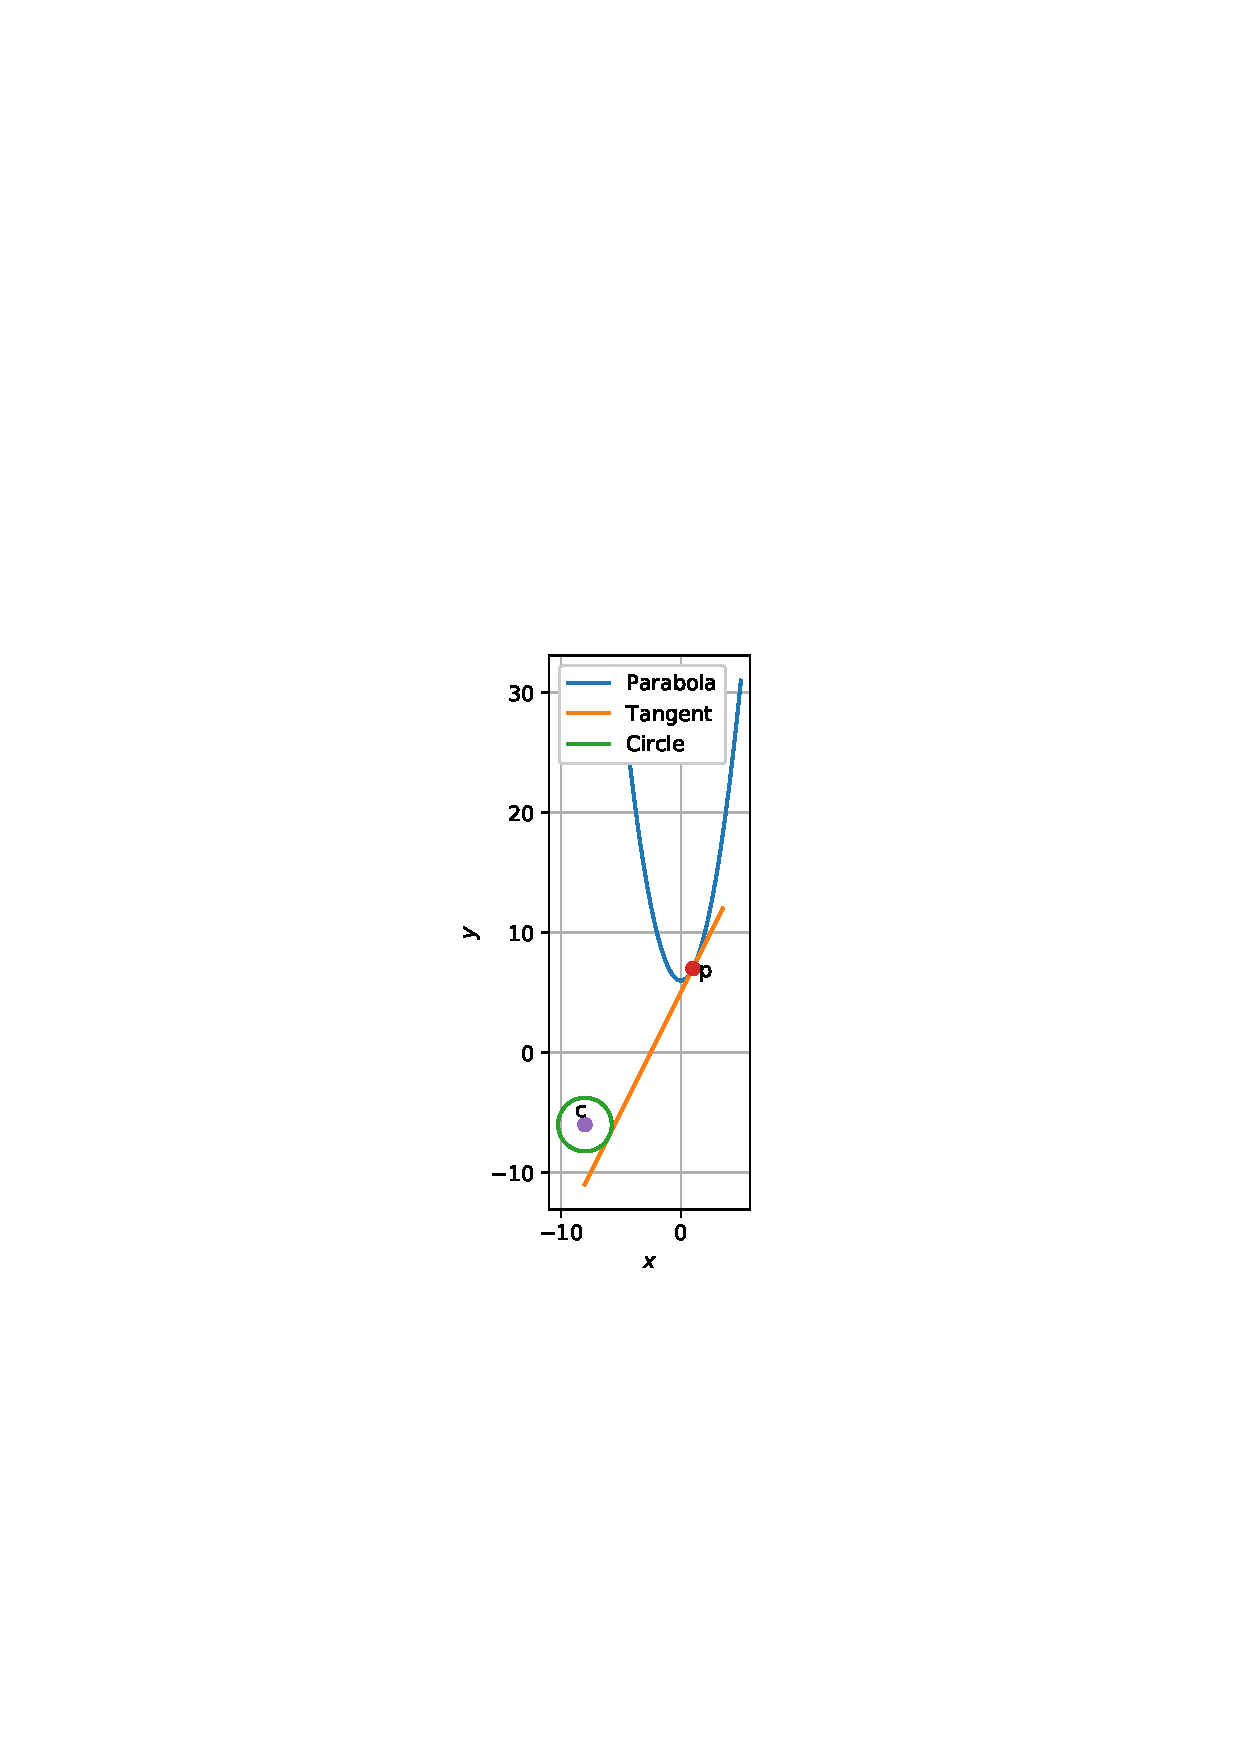
\includegraphics[width=\columnwidth]{./solutions/41/6/parab.png}
        \caption{Graph of $9x^2+24xy+16y^2-4y-x+7=0$}
        \label{eq:solutions/41/6/myfig}
\end{figure}
